\section{Theory}
\label{sec:theory}
This section aims to summarize the basic principles that underpin the operation of diode lasers.

\subsection{The Diode Laser}
\label{sec:diodelaser}
The term 'laser' stands for \textbf{L}ight \textbf{A}mplification by \textbf{S}timulated \textbf{E}mission of
\textbf{R}adiation. A laser is a unique source of electromagnetic radiation, characterized by
properties such as an extensive coherence length, monochromaticity, and concentrated intensity
paired with minimal divergence. Owing to these distinctive features, lasers are versatile and find
applications in various areas. Within this experiment, we employ a diode laser as a tool
for spectroscopic analysis.\\
\noindent
The operation of a laser amplifies radiation by the mechanism of stimulated emission. For a laser to function
effectively, stimulated emission must dominate over both absorption and spontaneous emission within the laser medium.
This is achieved through establishing population inversion. Additionally, an optical resonator is used to enhance the
emitted radiation further. \\
\\
\noindent
The laser device used in this experiment has at its core a semiconducting diode. It consists of at least three layers:
the active layer, the n-doped layer and the p-doped layer. In the n- and p-doped layer, free charge carriers in the
form of electrons and electron holes respectively, are present. The active layer of the laser diode forms a cavity. A
injection current is run through the diode, causing
the electrons and electron holes to recombinate in the active layer between the n- and p-doted layers.
Therefore, the wavelength of the emitted photons corresponds to the width of the band gap of the semiconductors
material. This process can also be caused by another photon; this process is called stimulated emission.
If the injection current is high enough, the amplification through stimulated emission exceeds the optical
losses in the diode and population inversion can be achieved. In this case, the diode emits a coherent beam.
The emitted radiation is confined by refraction to a channel inside the diode (the active layer), with facets at the
ends of the channel that serve as cavity mirrors and output couplers. The diode used in this experiment emits most
radiation through the front facet, as the back facet is for the most part reflective. A schematic display of such a
laser diode chip is given in Figure~\ref{fig:diode}.
\begin{figure}[H]
  \centering
  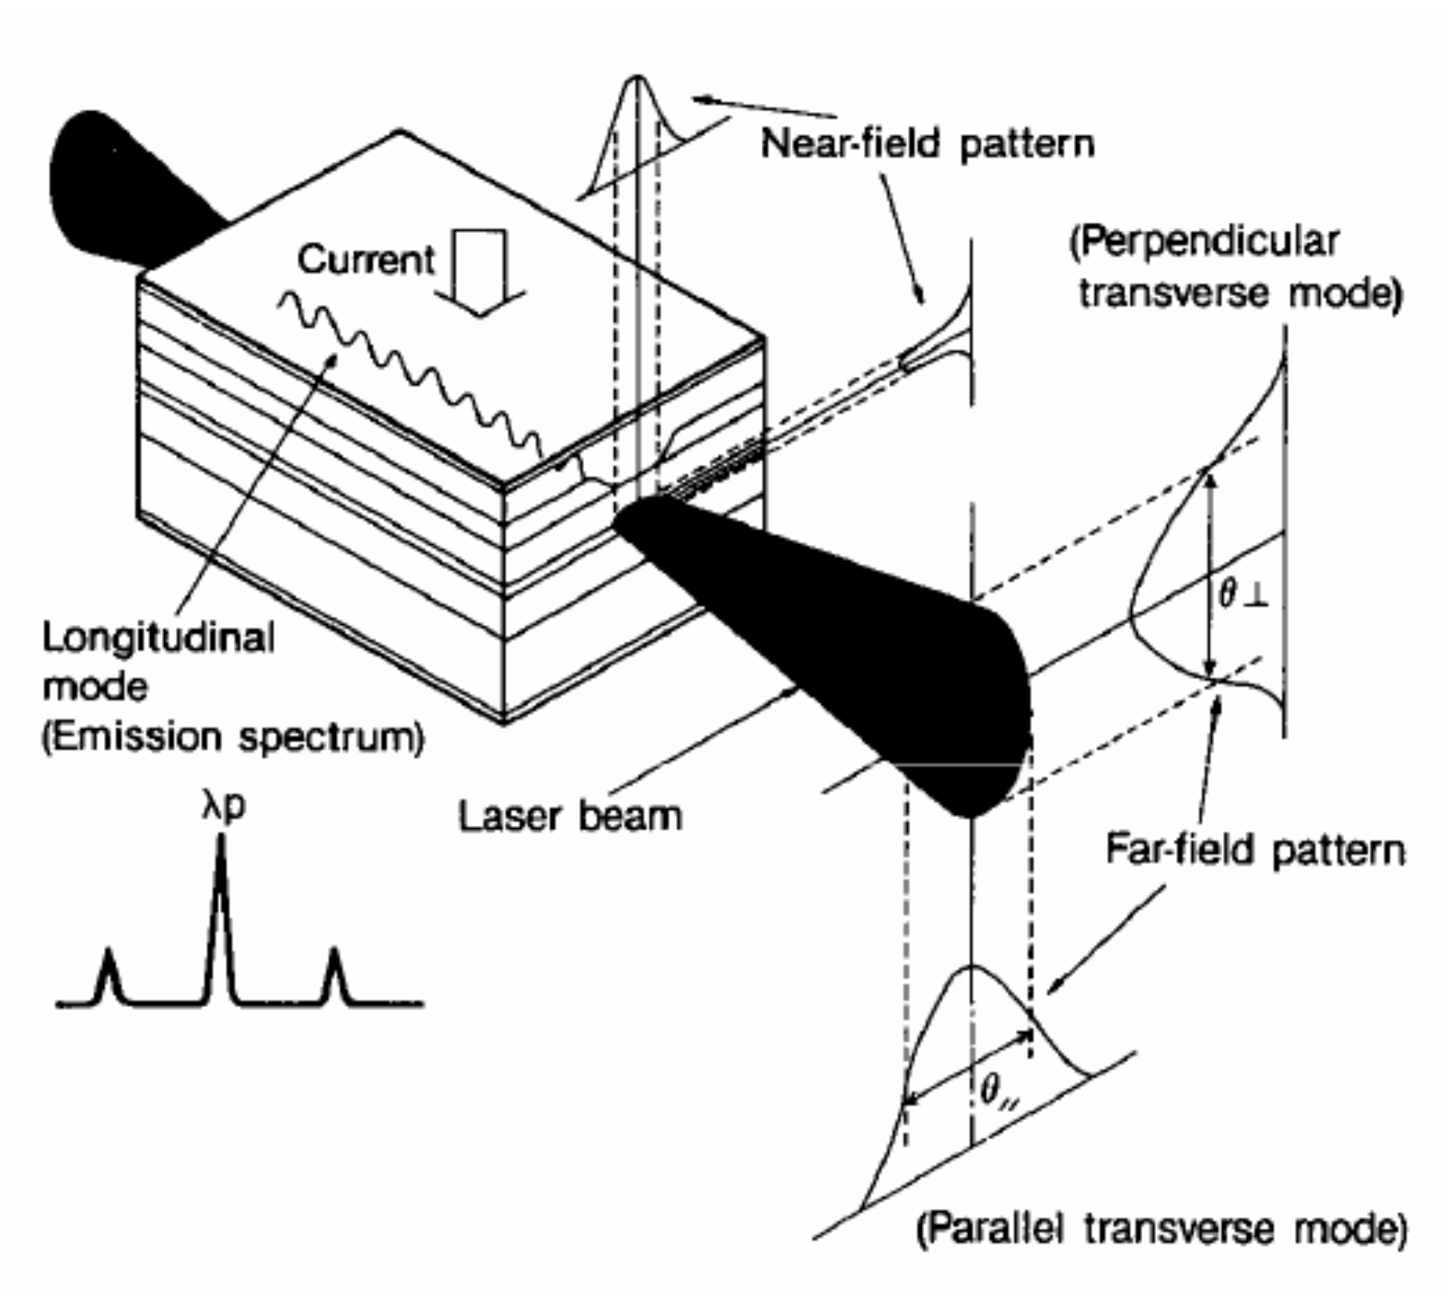
\includegraphics[scale=0.4]{./pictures/Diode-schematisch.png}
 \caption{Schematic display of a laser diode (LD) chip~\cite{teachspin}.}
 \label{fig:diode}
\end{figure}
\noindent
However, the light emitted by the raw laser diode chip has certain limitations; the beam is strongly diverging,
the frequency stability is very sensitive to optical feedback and the radiation has a linewidth of $~10$ times the
linewidth of atomic transitions. To overcome these problems, a configuration like the one displayed in
Figure~\ref{fig:laser-system} can be employed.
\begin{figure}
  \centering
  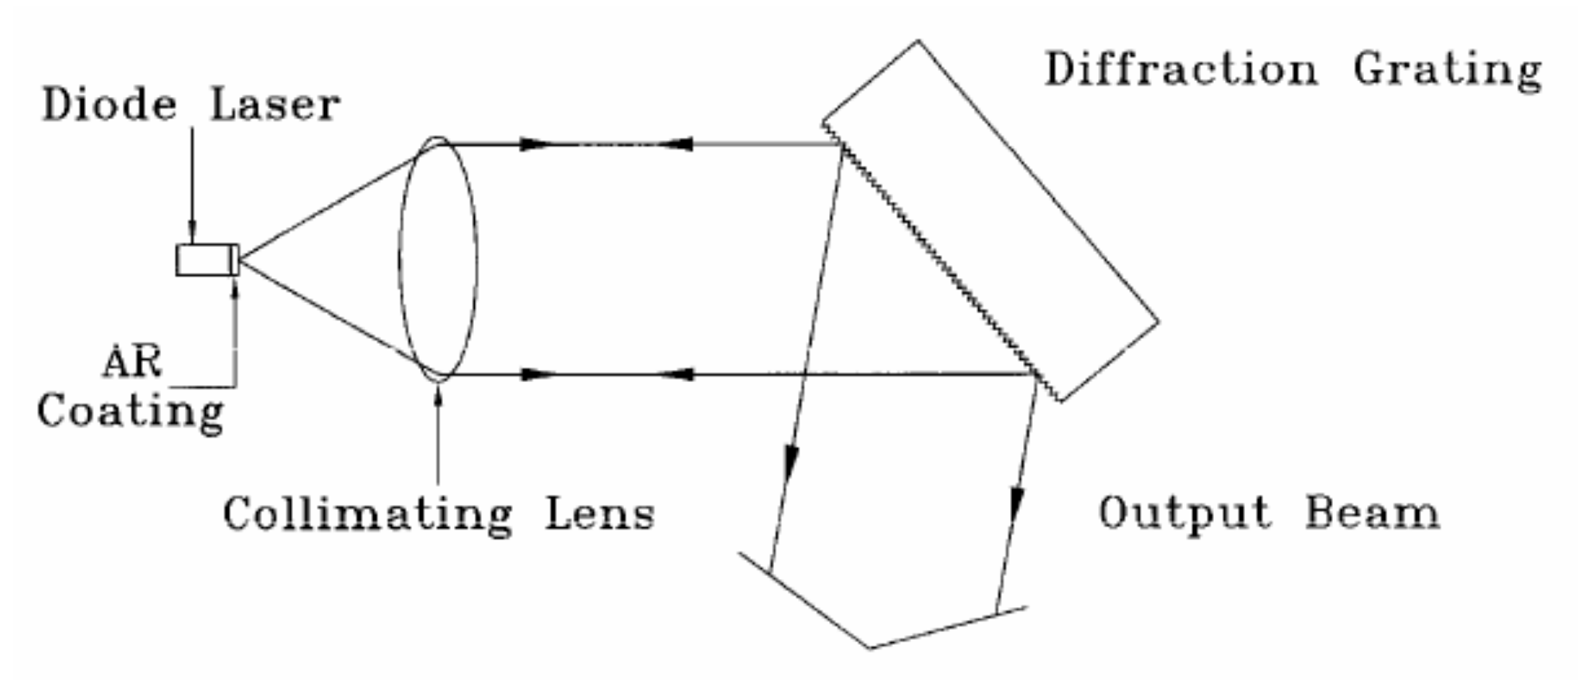
\includegraphics[scale=0.4]{./pictures/Laser-system.png}
  \caption{Configuration of a laser system~\cite{teachspin}.}
  \label{fig:laser-system}
\end{figure}
\noindent
Here, a collimating lens is used to prevent the divergence of the laser beam. To improve frequency stability,
around $\SI{15}{\percent}$ of light is routed back into the diode through the use of a diffraction grating.
This grating acts as an external cavity (in addition to the internal cavity inside the laser diode chip).
The grating also reduces the linewidth of the laser beam to less than $\nu = \SI{1}{\mega\hertz}$, which is
smaller than the atomic transitions linewidths.

\subsection{Tuning of the Diode Laser}
\label{sec:tuning}
After the lasing process has started, the beam mostly consists of light with the frequency that offers the highest
net optical gain. The exact frequency depends on several factors, which are displayed in
Figure~\ref{fig:diode-frequency}.
\begin{figure}
  \centering
  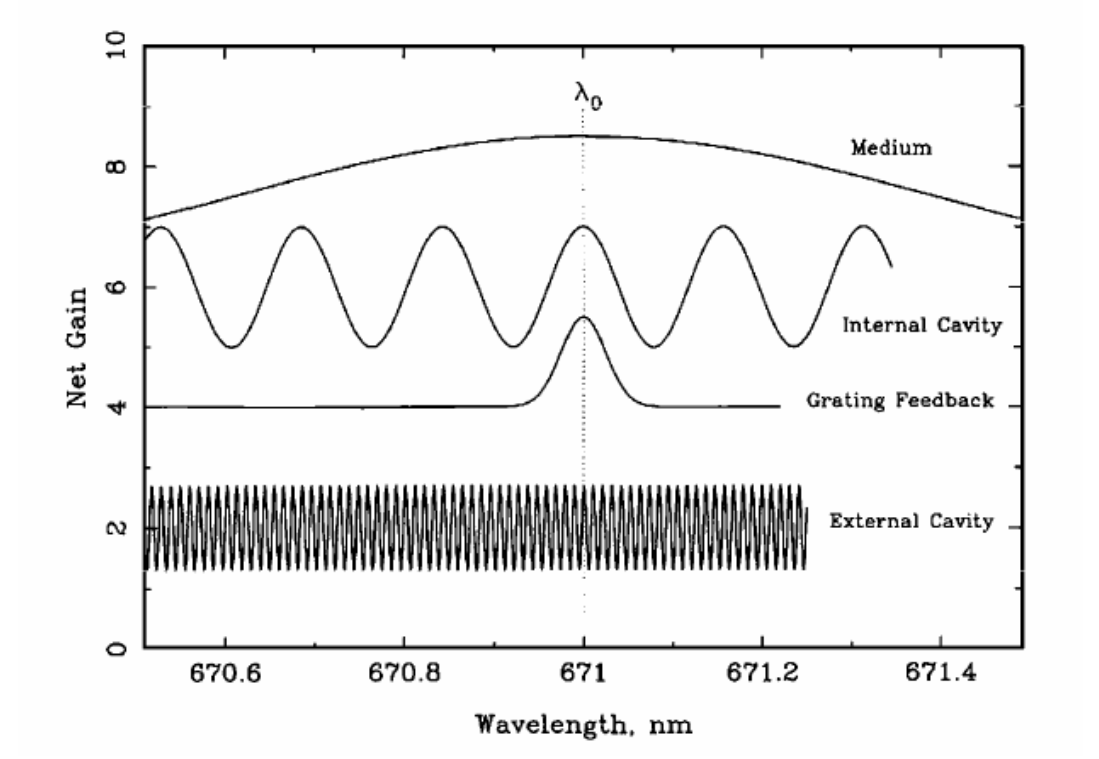
\includegraphics[scale=0.35]{./pictures/Diode-frequency.png}
  \caption{Schematic display of different sources of amplification for different wavelengths~\cite{teachspin}.}
  \label{fig:diode-frequency}
\end{figure}
\subsubsection{The Medium Gain}
\label{sec:mediumgain}
The medium gain pictured in Figure~\ref{fig:diode-frequency} is defined by the semiconductors material. It is
quite broad and is only influenced by the materials temperature, which can be used to shift the medium gain.
It is the least precise tuning parameter of a diode laser and should therefore be tuned at first.
\subsubsection{The Internal Cavity Gain}
\label{sec:internalcavitgain}
The gain caused by the internal cavity of the laser diode chip depends on the length of the cavity and the
injection current. Its periodic frequency is a result of the normal mode structure of the optical cavity; the
period length is defined by the length of the cavity, which is influenced by the temperature. \\
The temperature is then again influenced by the injection current; its strength changes both the cavity length
through temperature change as well as influencing the amount of charge carriers in the active layer.
\subsubsection{The optical Grating Gain}
\label{sec:opticalgratinggain}
The optical grating routes a small amount of radiation within a specific portion of the frequency band back
into the laser diode chip. The resulting singular peak can be seen in Figure~\ref{fig:diode-frequency}.
The position of this peak in the spectrum can be ajusted through a change in the angle of the optical grating.
Said adjustment can be done manually (e.g. with a screw) or though utilising a Piezo-electric crystal;
applying different voltages on such a crystal causes a proportional volume change, which can be converted into
a change of angle.
\subsubsection{The external Cavity Gain}
\label{sec:externalcavitygain}
The external cavity works similarly to the internal cavity gain, except its much larger cavity length: it is
confined by the reflective facet of the laser diode chip on one side and by the optical grating on the other.
As with the internal cavity gain, the length of the cavity determines the periodicity of the resulting
amplification. Because of its larger size, the external cavity gain is much shorter in its period length, as
can be seen in Figure~\ref{fig:diode-frequency}.
\subsubsection{Mode Hops}
\label{sec:modehops}
As mentioned before, after the lasing process has begun, the laser mostly emits radiation with the wavelength
that maximises the optical amplification. Adjusting the laser to a frequency where it emits the most radiation
continuously is complicated by mode hops, meaning a jump between different maxima in different gains.
When the angle of the optical grating is changed and therefore its gain is shifted, the total net gain also
depends on the other gain factors, like the internal cavity gain. The emitted frequency will then hop between
the maxima of the different gain factors. This can be seen in Figure~\ref{fig:hophop}.
\begin{figure}
  \centering
  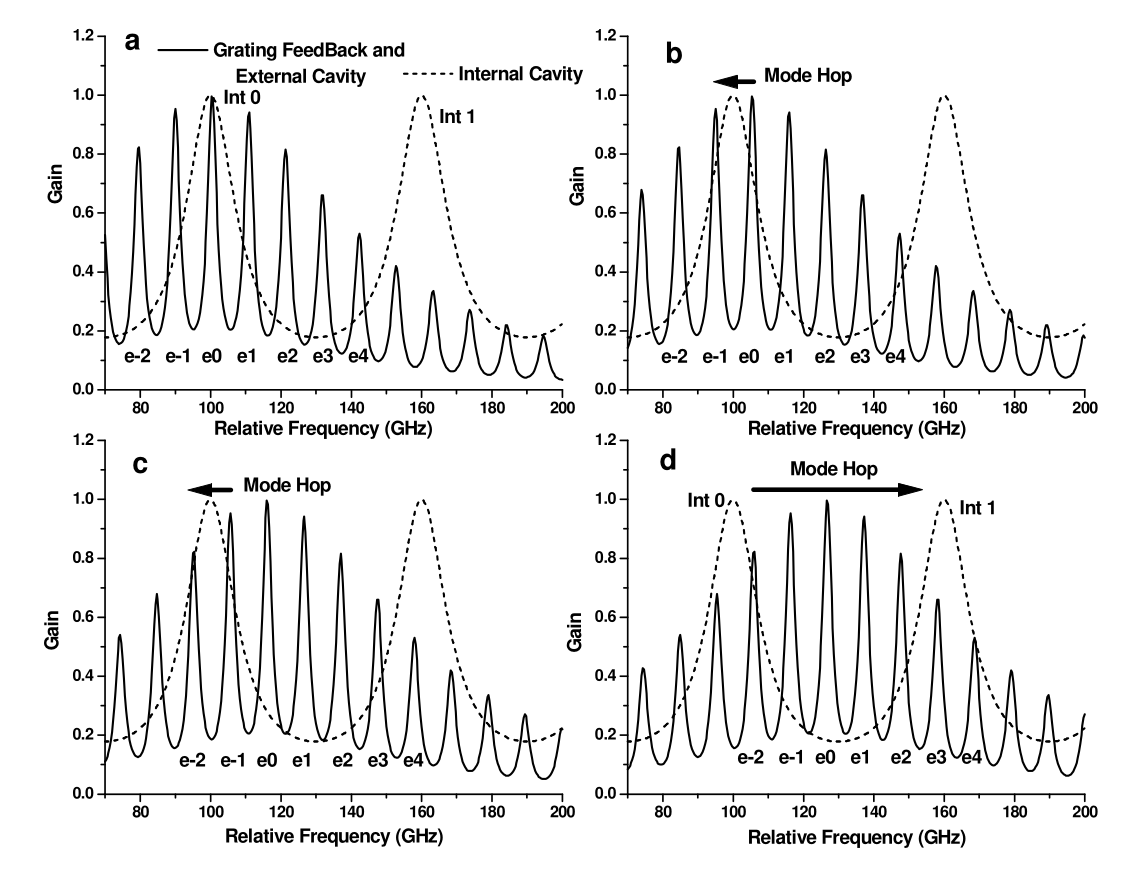
\includegraphics[scale=0.4]{./pictures/hophop.png}
  \caption{Several plots of the gain by the external cavity and the optical grating for different wavelengths~\cite{teachspin}.}
  \label{fig:hophop}
\end{figure}
To prevent mode hops, the gain factors have to be adjusted simultaneously.
